\section{随机游走}
\label{sec:graph-random-walk}

一步怎样选邻居，决定了多步以后棋子可能落在哪里。我们先从四点路径上的具体走步出发，明确一步选择的规则，再将所有可能行走的终点汇总为位置分布。

\subsection{随机游走}
\label{sec:graph-walk-rule}

在单位权路径$1\!-\!2\!-\!3\!-\!4$上，把棋子放在顶点$1$。顶点$1$只有一条边连到$2$，所以第一步别无选择，必须走到$2$。

到了$2$之后，面前有两条边：一条回到$1$，一条通往$3$。两条边的权重都是$1$，总共$2$。回到$1$的概率是$1/2$，走到$3$的概率也是$1/2$。如果把从$2$到$3$的边权提高为$3$，那么从$2$离开时两条边的权重共为$1+3=4$，回到$1$的概率变成$1/4$，走到$3$的概率变成$3/4$。选择概率始终由出发顶点的邻边权重决定。

\begin{definition}[随机游走]
\label{def:graph-random-walk}
记$X_t$为第$t$步所在的顶点。给定$X_t=i$，下一步选择$j$的概率与边权$w_{i,j}$成正比，
\begin{equation}
\mathbb{P}(X_{t+1}=j\mid X_0,\ldots,X_t)=\frac{w_{i,j}}{d_i}.
\label{eq:graph-walk-transition-rule}
\end{equation}
若$d_i=0$（孤立顶点），约定棋子停留在原地。
\end{definition}

这条\term{随机游走}（random walk）规则只读取当前位置。即使两次走到$i$的路线完全不同，从$i$出发的下一步概率仍然一样。

用$\nu_i^{(t)}=\mathbb{P}(X_t=i)$记第$t$步在顶点$i$的概率，把各点的概率排成一行，记作$\bm{\nu}^{(t)}$。下标$i$指定顶点，上标$(t)$指定时刻。$\bm{\nu}^{(0)}$就是起点分布。

一条给定的行走序列$v_0,v_1,\ldots,v_k$要求棋子先出现在$v_0$，再依次完成各步转移。每接上一步，就把此前走完该前缀的概率乘上这一跳的转移概率。因此这条行走的概率为
\begin{equation}
\mathbb{P}(X_0=v_0,\ldots,X_k=v_k)
=\nu^{(0)}_{v_0}\prod_{j=0}^{k-1}\frac{w_{v_j,v_{j+1}}}{d_{v_j}}.
\label{eq:graph-walk-path-probability}
\end{equation}

回到单位权路径。从$1$出发，$1\to2\to1$的概率是$1\cdot(1/2)=1/2$，$1\to2\to3$的概率也是$1\cdot(1/2)=1/2$。两条路径走了相同的步数，但中途经过不同的顶点。若包含孤点，对应因子按停留规则取$1$。

\subsection{多步分布}
\label{sec:graph-walk-distributions}

上面计算了单条路径的概率。如果要问"第$t$步落在顶点$j$的概率是多少"，就需要把所有在第$t$步到达$j$的路径概率加起来。转移矩阵把这个求和变成一次矩阵乘法。

\paragraph{转移矩阵}

把从每个顶点出发的一步选择概率排成一行，再把$n$行叠起来，就得到\term{转移矩阵}（transition matrix）$\bm{P}$。第$i$行记录从$i$出发到各点的概率，第$j$列收集各处走到$j$的概率。设加权邻接矩阵为$\bm{W}=(w_{i,j})$，把$\bm{W}$的第$i$行除以$d_i$，等于在左侧乘$\bm{D}^{-1}$，于是
\begin{equation}
\bm{P}=\bm{D}^{-1}\bm{W}.
\label{eq:graph-walk-transition-matrix}
\end{equation}
矩阵元素非负，每行之和为$1$，即$\bm{P}\bm{1}=\bm{1}$。

\paragraph{一步更新}

要算第$t+1$步到达$j$的概率，可以按上一步所在的位置$i$分类。棋子在第$t$步落在$i$的概率是$\nu_i^{(t)}$，从$i$一步到$j$的概率是$P_{i,j}$。把这两个概率相乘再对所有$i$求和，就得到
\begin{equation}
\nu^{(t+1)}_j=\sum_i \nu^{(t)}_i P_{i,j}.
\label{eq:graph-walk-distribution-entry}
\end{equation}

这个求和就是概率行$\bm{\nu}^{(t)}$右乘$\bm{P}$的第$j$个分量。每多走一步，右边就多乘一个$\bm{P}$，从而
\begin{equation}
\bm{\nu}^{(t+1)}=\bm{\nu}^{(t)}\bm{P},
\qquad
\bm{\nu}^{(t)}=\bm{\nu}^{(0)}\bm{P}^t.
\label{eq:graph-walk-distribution}
\end{equation}
取初始分布为顶点$u$上的点质量，$\bm{P}^t$的第$u$行就是第$t$步的分布。

\paragraph{四点路径的前四步}

在单位权路径$1\!-\!2\!-\!3\!-\!4$上，四个顶点的度分别为$1,2,2,1$。转移矩阵为
\[
\bm{P}=\begin{pmatrix}
0&1&0&0\\
1/2&0&1/2&0\\
0&1/2&0&1/2\\
0&0&1&0
\end{pmatrix}.
\]
从顶点$1$出发，初始行只有第一个分量为$1$。第一次乘$\bm{P}$时，只读取$\bm{P}$的第一行，所以一步后全部质量集中在顶点$2$。

第二次乘$\bm{P}$时读取第二行。顶点$2$的$1/2$概率回到$1$，$1/2$概率走到$3$。第三次乘$\bm{P}$时，分别取$\bm{P}$的第一行和第三行各乘$1/2$再相加。包含初态的计算结果为
\[
\begin{array}{c@{\qquad}c}
t&\bm{\nu}^{(t)}\\
0&(1,0,0,0)\\
1&(0,1,0,0)\\
2&(1/2,0,1/2,0)\\
3&(0,3/4,0,1/4)
\end{array}
\]
图~\ref{fig:graph-walk-path-distribution}把各步连起来。顺着顶点$2$在$t=3$处接到的两条箭头往回看，$3/4$中有$1/2$来自顶点$1$（经路线$1\to2$），另有$1/4$来自顶点$3$（经路线$3\to2$）。

图~\ref{fig:graph-walk-bar-chart}以柱状图展示同一组分布。每个面板对应一个时刻，柱高是当前在各顶点的概率。观察概率如何从起点逐步向路径的另一端扩散：$t=1$时质量全部集中在$2$，$t=2$时分到$1$和$3$，$t=3$时已传到$4$。

\begin{figure}[!htb]
\centering
\begin{tikzpicture}[x=1mm,y=1mm,
  bar/.style={fill=FigureBlueFill,draw=FigureBlue,line width=.45pt},
  panel/.style={anchor=mid,font=\figurefont\footnotesize},
  vlabel/.style={font=\figurefont\fontsize{7.5}{9}\selectfont,FigureInk,anchor=north},
  plabel/.style={font=\figurefont\fontsize{7}{8.5}\selectfont,FigureInk,anchor=south}]
  \def\barw{4}
  \def\barscale{20}
  \def\gap{3}
  % Panel t=1: (0,1,0,0)
  \begin{scope}[xshift=0mm]
    \draw[FigureStroke,line width=.4pt] (0,0) -- (0,\barscale+2);
    \draw[FigureStroke,line width=.4pt] (0,0) -- (4*\barw+3*\gap+1,0);
    \foreach \i/\v/\p in {0/1/0, 1/2/1, 2/3/0, 3/4/0} {
      \pgfmathsetmacro{\x}{\i*(\barw+\gap)+1}
      \pgfmathsetmacro{\h}{\p*\barscale}
      \ifnum\p>0
        \fill[bar] (\x,0) rectangle +(\barw,\h);
        \node[plabel] at (\x+\barw/2,\h) {$\p$};
      \fi
      \node[vlabel] at (\x+\barw/2,-1) {$\v$};
    }
    \node[panel] at (16,-8) {(a) $t=1$};
  \end{scope}
  % Panel t=2: (1/2,0,1/2,0)
  \begin{scope}[xshift=38mm]
    \draw[FigureStroke,line width=.4pt] (0,0) -- (0,\barscale+2);
    \draw[FigureStroke,line width=.4pt] (0,0) -- (4*\barw+3*\gap+1,0);
    \foreach \i/\v/\p/\plbl in {0/1/0.5/{1/2}, 1/2/0/{}, 2/3/0.5/{1/2}, 3/4/0/{}} {
      \pgfmathsetmacro{\x}{\i*(\barw+\gap)+1}
      \pgfmathsetmacro{\h}{\p*\barscale}
      \pgfmathparse{\p>0?1:0}
      \ifnum\pgfmathresult=1
        \fill[bar] (\x,0) rectangle +(\barw,\h);
        \node[plabel] at (\x+\barw/2,\h) {$\plbl$};
      \fi
      \node[vlabel] at (\x+\barw/2,-1) {$\v$};
    }
    \node[panel] at (16,-8) {(b) $t=2$};
  \end{scope}
  % Panel t=3: (0,3/4,0,1/4)
  \begin{scope}[xshift=76mm]
    \draw[FigureStroke,line width=.4pt] (0,0) -- (0,\barscale+2);
    \draw[FigureStroke,line width=.4pt] (0,0) -- (4*\barw+3*\gap+1,0);
    \foreach \i/\v/\p/\plbl in {0/1/0/{}, 1/2/0.75/{3/4}, 2/3/0/{}, 3/4/0.25/{1/4}} {
      \pgfmathsetmacro{\x}{\i*(\barw+\gap)+1}
      \pgfmathsetmacro{\h}{\p*\barscale}
      \pgfmathparse{\p>0?1:0}
      \ifnum\pgfmathresult=1
        \fill[bar] (\x,0) rectangle +(\barw,\h);
        \node[plabel] at (\x+\barw/2,\h) {$\plbl$};
      \fi
      \node[vlabel] at (\x+\barw/2,-1) {$\v$};
    }
    \node[panel] at (16,-8) {(c) $t=3$};
  \end{scope}
\end{tikzpicture}
\caption{从顶点$1$出发在四点路径上的前三步位置分布。柱高表示当前在各顶点的概率。$t=1$时全部质量在$2$。$t=2$时分成两半回到$1$和前进到$3$。$t=3$时已到达端点$4$，但$3/4$的质量留在$2$。}
\label{fig:graph-walk-bar-chart}
\end{figure}

\begin{BookInlineFigure}
\centering
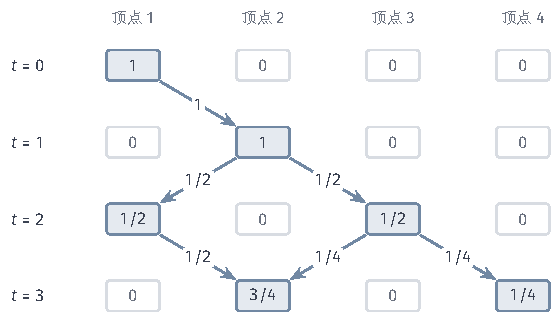
\includegraphics[width=94.132mm]{figures/03-graphs/05-matrices-and-spectra/tikz/walk-examples/path-distribution.pdf}
\caption{单位权路径$1\!-\!2\!-\!3\!-\!4$上从顶点$1$出发的分布。每行对应一个时刻，格内是当前位置的概率，箭头上的数字是这一小股概率在一步中实际转移的量。}
\label{fig:graph-walk-path-distribution}
\end{BookInlineFigure}

\paragraph{与邻接矩阵幂的关系}

第~\ref{chap:graph-adjacency-matrix}章用邻接矩阵$\bm{A}$的幂$(\bm{A}^t)_{u,v}$来计算从$u$到$v$的$t$步行走条数。在无权$d$正则图上，每个顶点的度都是$d$，每一步沿指定边行走的概率为$1/d$。同一条$t$步行走的概率为$d^{-t}$，因此
\[
\bm{P}^t=d^{-t}\bm{A}^t.
\]
度随顶点变化时，同样长的行走可有不同概率，上式不再成立。例如在四点路径上，从顶点$2$出发，$2\to1\to2$的概率是$(1/2)\cdot1=1/2$，$2\to3\to2$的概率是$(1/2)\cdot(1/2)=1/4$。两条路径长度相同，但经过不同度数的顶点，概率不一样。
